\documentclass[11pt]{jarticle}

%パッケージ
\usepackage{amsmath} % already loaded in the beginning of the main file
\usepackage{nccmath} 
\usepackage{amsfonts}
\let\openbox\undefined
\usepackage{amsthm} %% NOTE: incompatible with IPSJ class
\let\Bbbk\relax % fix \Bbbk problem in ACM class
\usepackage{amssymb}
\usepackage{mathtools} % \Coloneqq
\usepackage{stmaryrd} % \llparenthesis & rrparenthesis
\usepackage{ebproof}
\usepackage{nicefrac}
\usepackage{float} % \begin{figure}[H]
\usepackage[dvipsnames]{xcolor}
%\usepackage{amssymb,amsmath}
\usepackage{listings}
\usepackage[dvipdfmx]{graphicx}
\usepackage{enumerate}
\usepackage[hyphens]{url}
%\usepackage{amsfonts}
%\usepackage{mathtools}
%\usepackage{stmaryrd}

%\usepackage{multicol}
%レイアウト
\setlength{\oddsidemargin}{0mm}
\setlength{\textwidth}{160mm}
\setlength{\topmargin}{-9mm}
\setlength{\headheight}{0mm}
\setlength{\textheight}{241mm}
\lstset{
  basicstyle={\ttfamily},
  identifierstyle={\small},
  commentstyle={\smallitshape},
  keywordstyle={\small\bfseries},
  ndkeywordstyle={\small},
  stringstyle={\small\ttfamily},
  frame={tb},
  breaklines=true,
  columns=[l]{fullflexible},
  numbers=left,
  xrightmargin=0zw,
  xleftmargin=0zw,
  numberstyle={\scriptsize},
  stepnumber=1,
  numbersep=1zw,
  lineskip=-0.8ex
}

%コマンド
\newcommand{\projection}[2]{{\color{cyan}\llparenthesis}#1{\color{cyan}\rrparenthesis^#2}}
%\newcommand{\gray}[1]{\textbf{\textsf{\color{Gray}#1}}}
\newcommand{\cyan}[1]{\color{cyan}#1}
%\lstset{
%  language=Lisp,
%  frame=tblr,
%  commentstyle=\ttfamily,
%  morekeywords={
%    if, define
%  }
%}
%%%%%%%%%%%%%%%%%%%%%%%%%%%%%%%%%%%%%%%%%%%%%%%%%%
\begin{document}
%\bibliographystyle{jplain}
%%%%%%%%%%%%%%%%%%%%%%%%%%%%%%%%%%%%%%%%%%%%%%%%%%
%%% Header
\begin{flushleft}
  中間発表\hspace{\fill}
  恩田晴登 (2023年7月25日)
\end{flushleft}
\begin{center}
{\Large\bf Pythonの静的型検査器を活用したコレオグラフィックプログラミング言語の実装}
\end{center}

%%%%%%%%%%%%%%%%%%%%%%%%%%%%%%%%%%%%%%%%%%%%%%%%%%
\section{研究背景}
コレオグラフィー\cite{choreography}は,プログラマーが通信のロールごとに振舞いを個別に定義するのではなく,ロール間で
どのように通信が起こるのかといった全体像を示すマルチパーティプロトコルである.
コレオグラフィーで各ロールの動作を相互的に定義しているため,デッドロックや競合状態
などの並行性に起因するエラーが起こらないことは保証されており,各ロールの具体的な実装は
コレオグラフィーに従って記述することで安全性が保たれている.しかし,分散システムにおける
各ロールのプログラミングをする際は,相互作用する複数のプログラムを正しく調整しながら記述する
必要があり,手動で制御(channelを介して送信・受信)するのはプログラマーの大きな負担となる.

先行研究で開発されたコレオグラフィックプログラミング言語である{\bf{Choral}}\cite{choral}は,
分散システムに従わせたいプロトコル全体を単一のプログラムとして作成できるため,
プログラマーの負担を軽減する.ChoralはJavaに新しい型{\bf{$T@(R_1,\cdots,R_n)$}}
を加えて拡張した言語であり,これによって相互的な通信が各ロール間でどのように行われているかが
分かるようになる.さらに,Choralで記述したコレオグラフィーをコンパイルすると,ロールごとの
Javaライブラリに変換されて自動生成されて,各プログラムは全体のプロトコルに正しく従う.
% Choralの例
\begin{figure}[htbp]
  \begin{center}
  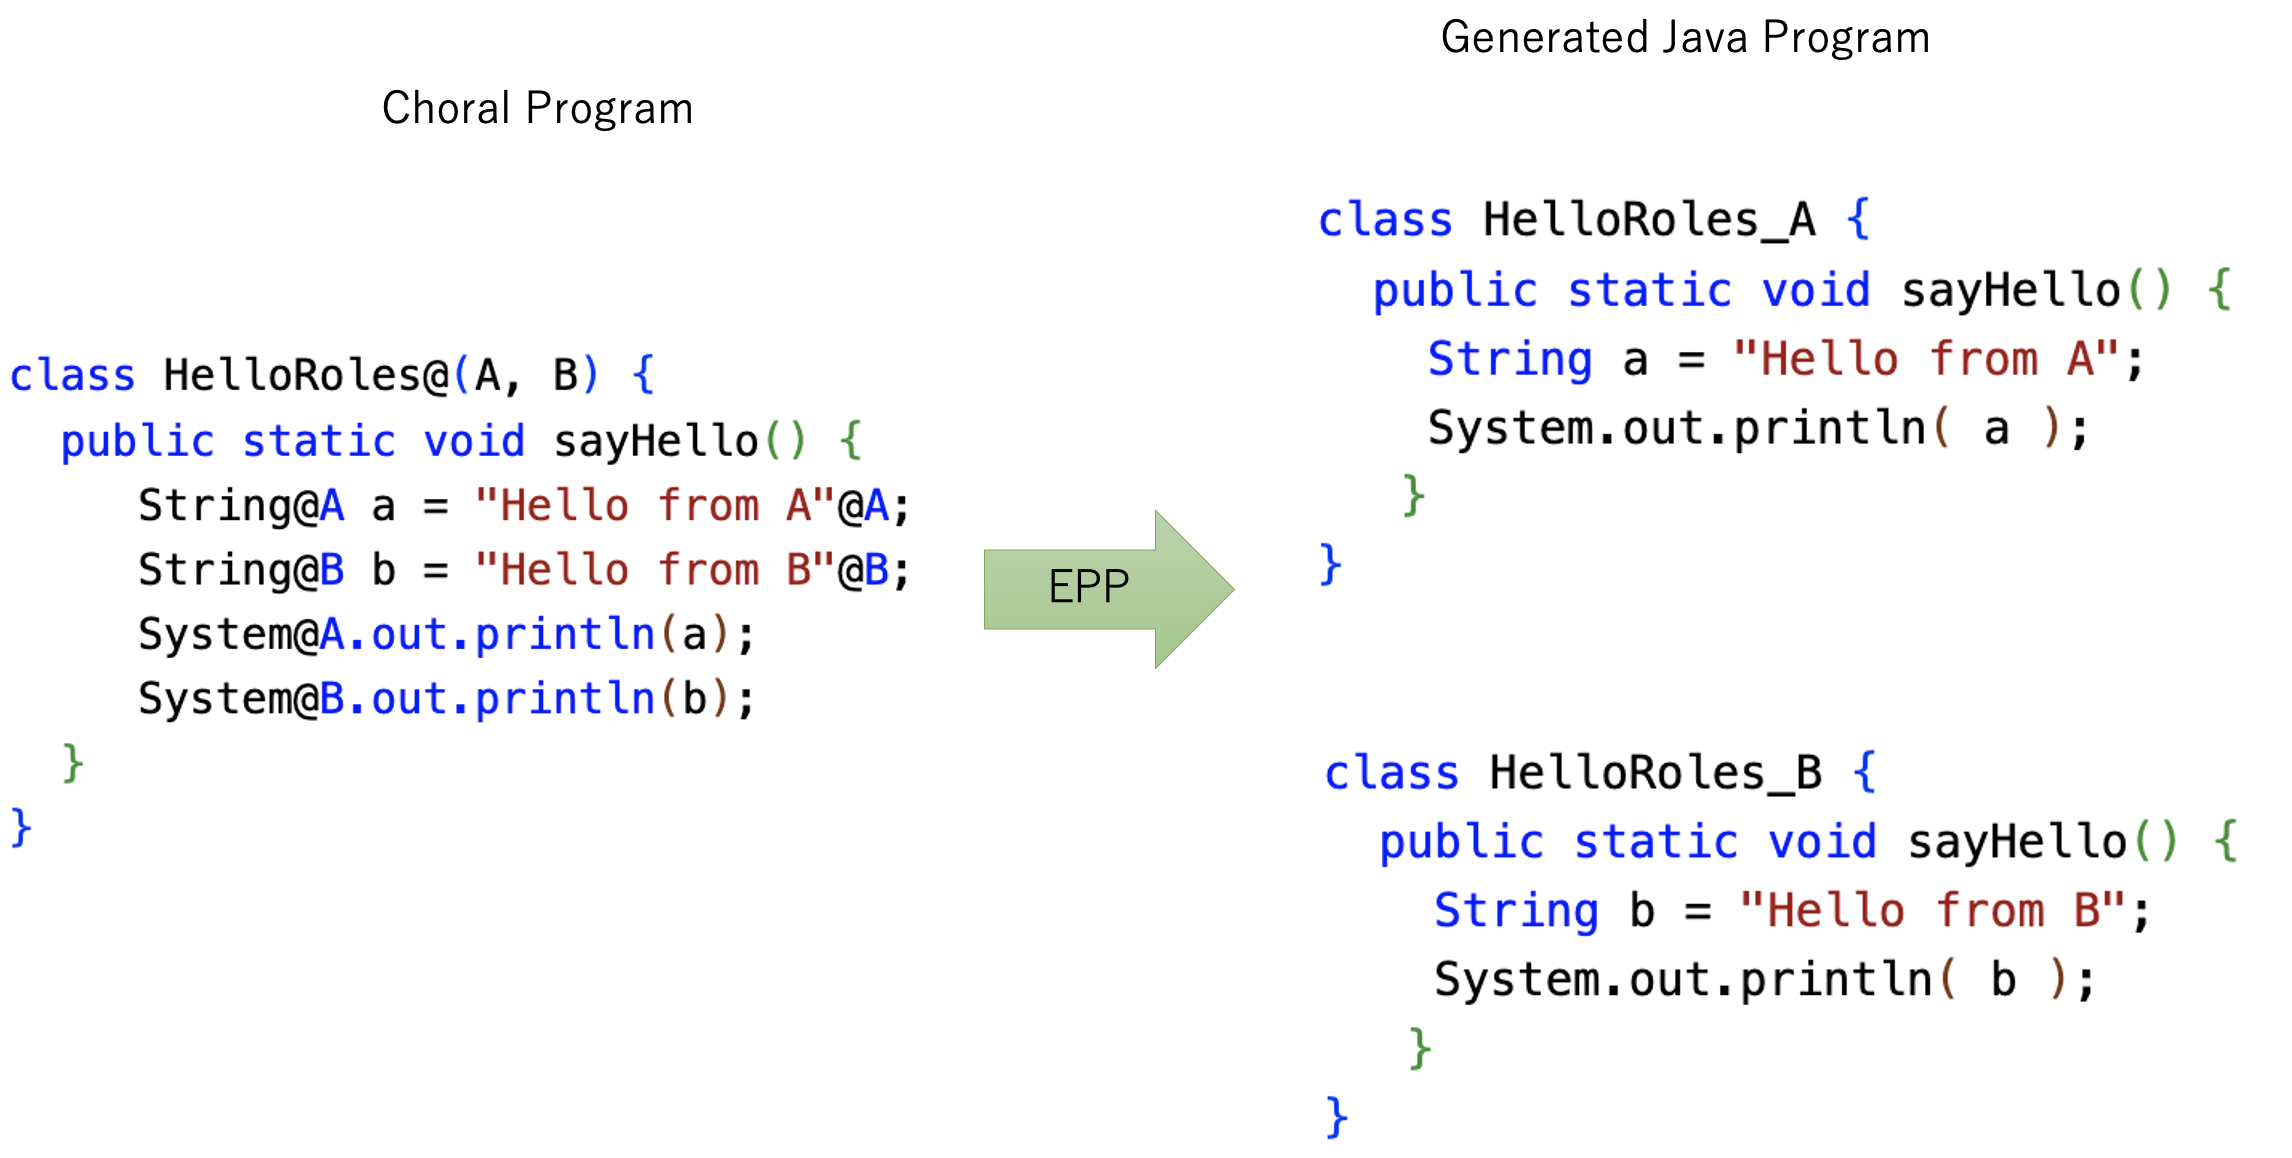
\includegraphics[width=130mm]{choral_ex.png}
  \caption{Choralの例}
  \end{center}
\end{figure}

コンパイル時にコレオグラフィーからエンドポイントのプログラムを自動生成する研究はJava以外の言語を拡張した場合も実装できるのではないかと考え,
本研究ではJavaを拡張したChoralを参考に,Pythonを拡張したコレオグラフィックプログラミング言語であるPyChoralの開発を行う.
%%%%%%%%%%%%%%%%%%%%%%%%%%%%%%%%%%%%%%%%%%%%%%%%%%
\newpage
\section{研究概要}
本研究はコレオグラフィーを用いて分散システムを記述するプログラマーの負担を軽減することを目的として,Pythonを拡張したPychoralの開発をする.
ここで,Choralの拡張元であるJavaが静的型付け言語であることに対してPythonは動的型付け言語であるため,コンパイル時に型情報から発生するエラーは生じない.この問題を解決するために,
Pythonに標準的に備わっている静的型検査器である{\bf{Mypy}}\cite{mypy}を使用してプログラムの実行前にエラーの有無を確認できるようにする.
MypyはPythonプログラムに型注釈をつけて,その情報をもとにコンパイル時に型検査を行う.

しかし,Mypyを用いてPythonをJavaと同じように拡張すればいいかと言うと,問題がある.
Choralの型検査では$@$の後ろに型として記述されているロールの型情報をもとに各ロールのプログラムに射影していたのだが,Mypyには
$@$でロールの情報をとる機能はあらかじめ備わっていない.
そこで,本研究ではPythonのobjectクラスに$@$のためのメソッドを追加する.
例えば,$123@A$と記述した場合{\bf{$\text{At}[\text{int,A()}]$}}という型情報が得られる.
PyChoralでは構文解析時にこの{\bf{At}}型が現れたらリストの第二引数からロールの情報を取得できる.

PyChoralはMypyの内部機能によって一度構文木を構築し,visitorパターンによって射影するロールの情報を持ちながら構文木をトラバースし,射影の定義
に従って各ロールのPythonプログラムを文字列として生成する.

\begin{figure}[htbp]
  \begin{center}
  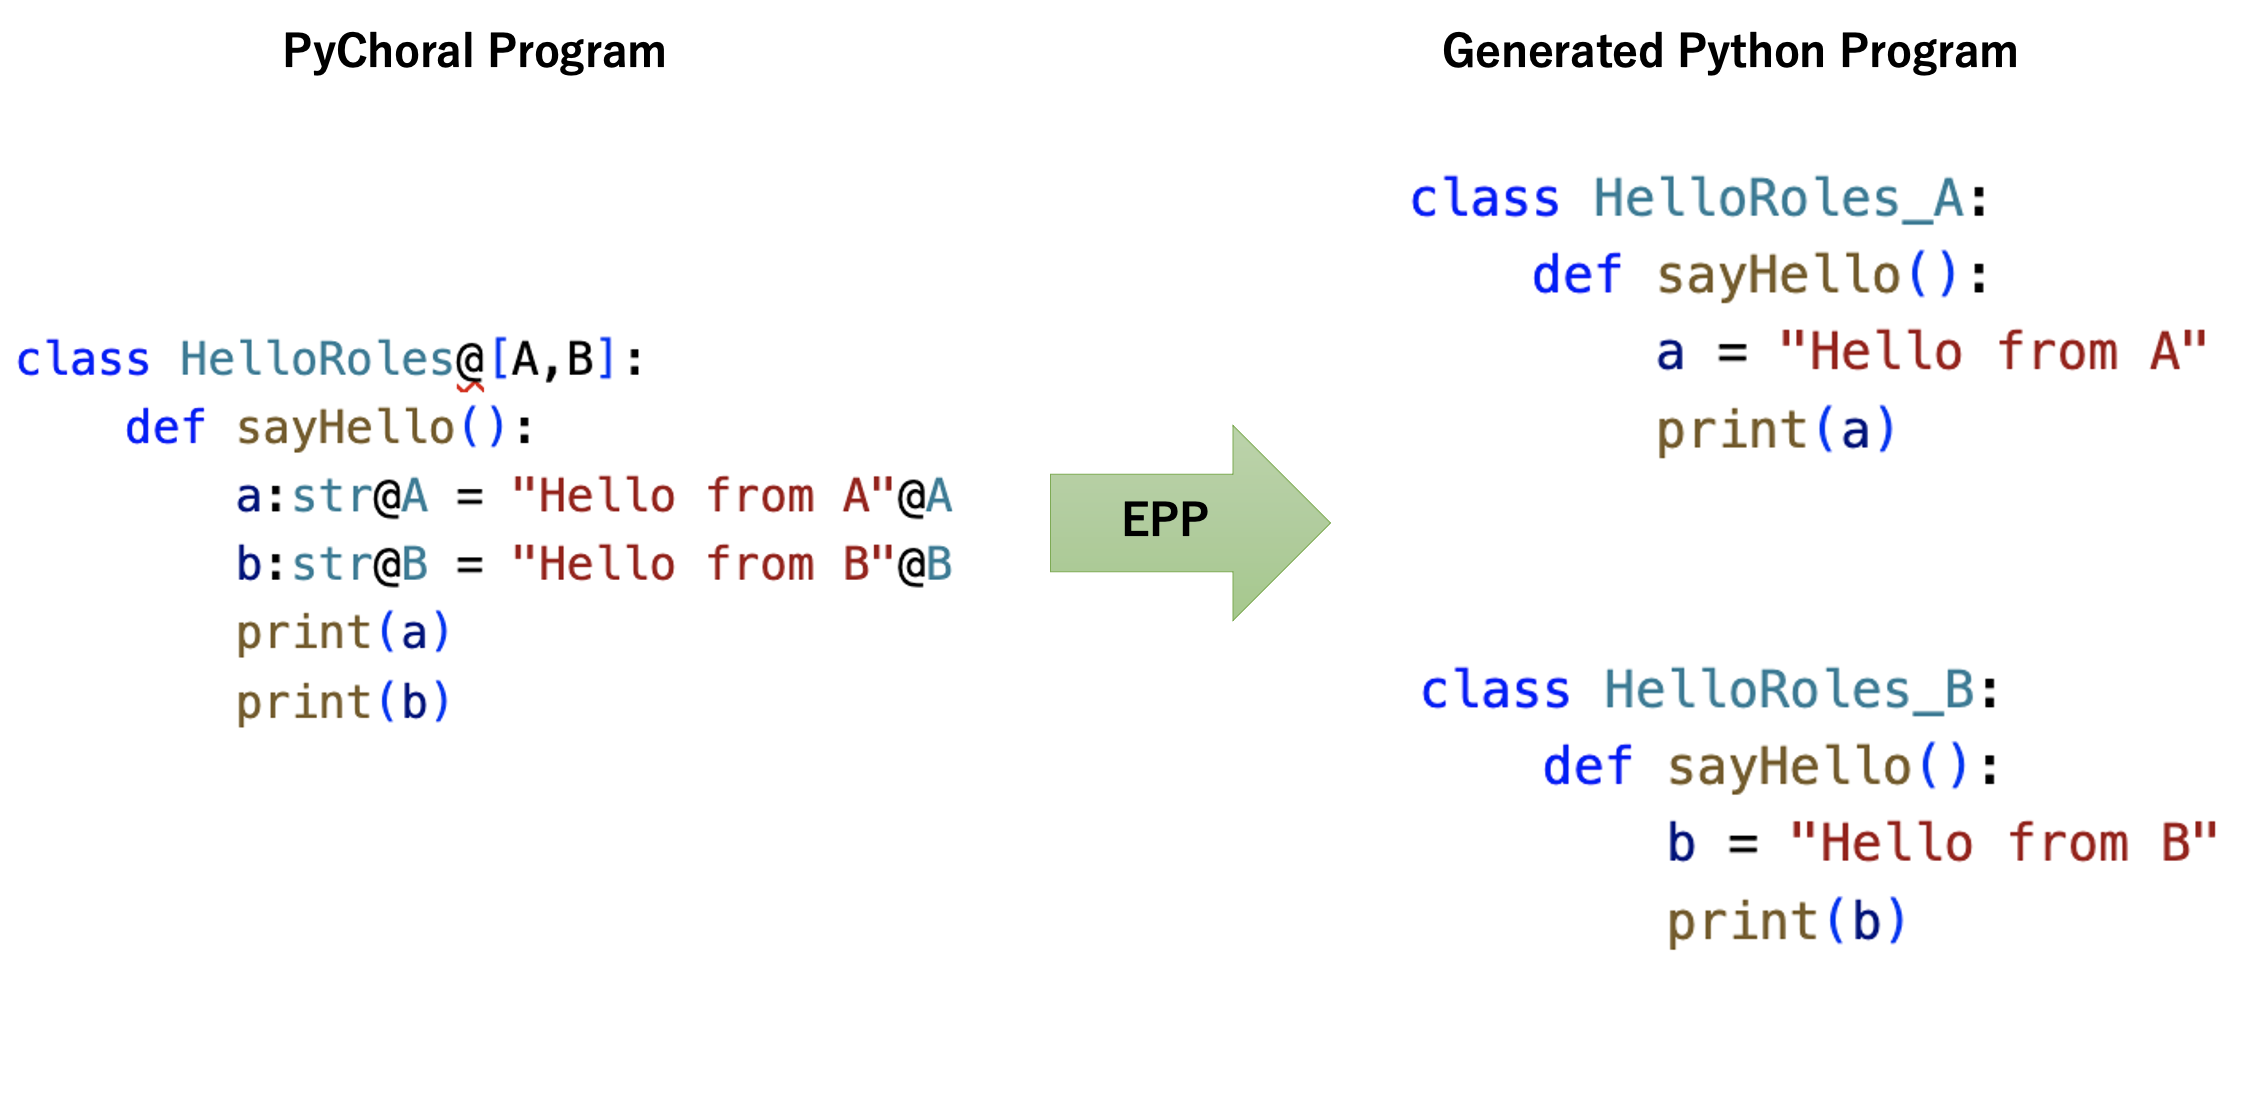
\includegraphics[width=130mm]{Pychoral_ex.png}
  \caption{PyChoral(完成後)の例}
  \end{center}
\end{figure}

%%%%%%%%%%%%%%%%%%%%%%%%%%%%%%%%%%%%%%%%%%%%%%%%%%
\section{進捗}
Pythonのプログラムのうち式(Expression)に対して構文・射影の定義,実装をした
(ただし,PyChoralのプログラムを射影した結果を出力するのみ).

例として,メソッド呼び出し$\texttt{ch}_\texttt{AtoB}.\texttt{comm(1@A):int@B}$
の射影後のプログラムの実装を紹介する.
$\texttt{ch}_{\texttt{AtoB}}$はロール$\texttt{A,B}$間のチャネルを表し,$\texttt{comm}$は
あるロールからもう一方のロールに引数の値を渡すメソッドである.例の場合,ロールAが
ロールBに対して$\texttt{int}$型の値をチャネルを介して送信していることになる.
これをロールA,ロールB,この通信に関係ないロールCに対して,本研究で定義した方式で射影した結果を以下に示す.
ただし,$\projection{Term}{A}$はロールAに対する項の射影を表すとする.
\begin{align*}
  &\projection{\texttt{ch}_\texttt{AtoB}.\texttt{comm(1@A):int@B}}{A} = \texttt{Unit.id(}\texttt{ch}_\texttt{AtoB}.\texttt{comm(1))}\\
  &\projection{\texttt{ch}_\texttt{AtoB}.\texttt{comm(1@A):int@B}}{B} = \texttt{ch}_\texttt{AtoB}.\texttt{comm(\texttt{Unit.id})}\\
  &\projection{\texttt{ch}_\texttt{AtoB}.\texttt{comm(1@A):int@B}}{C} = \texttt{Unit.id}
\end{align*}
ロールAの場合,チャネルと$\texttt{comm}$の引数に関わっているが,メソッド呼び出し自体の戻り値としては関与していないため,呼び出しだけを残した形でロールAのPythonプログラムに射影される.
ロールBの場合,戻り値の型情報で出てきているため式は残るが,$\texttt{comm}$の引数の型情報としてロールBの情報は取れないため,引数はUnit値となる.ロールCの場合,通信を行うチャネルに関与してないため,
ロールCのプログラムにはこのメソッド呼び出しは記述されない.
$\texttt{Unit.id}$と射影された後,その値をプログラム中から消すかどうかはNormalizerで処理するため,現在考察中である.

このように,構文や射影方式の定義を基にして式だけでなく文やクラス定義などを実装することで,Choralと同様に,
コレオグラフィーから振り付け規則を遵守したエンドポイントのPythonプログラムを生成する言語の開発を進める.
%%%%%%%%%%%%%%%%%%%%%%%%%%%%%%%%%%%%%%%%%%%%%%%%%%
\section{今後の課題}
\begin{itemize}
  \item 引き続きPyChoralの構文定義と実装を行う
  \item Merging,Normalizerの理解を深める
  \item 現段階ではPyChoralプログラムから射影されたPythonプログラム
  を文字列として出力しているだけであるため,これらを新たなファイルとして
  生成するように変更する.
  \item PyChoralを用いて分散システムのプログラム例をいくつか示す.
  
  (例:分散認証システム,クイックソート,マージソート)
\end{itemize}
%%%%%%%%%%%%%%%%%%%%%%%%%%%%%%%%%%%%%%%%%%%%%%%%%%
\begin{thebibliography}{99}
  \bibitem{choreography}Saverio Giallorenzo, Fabrizio Montesi and Marco Peressotti. 
  Object-Oriented Choreographic Programming, 2022.

  \bibitem{choral} Choral.    https://www.choral-lang.org/index.html
  
  \bibitem{mypy} mypy.   https://mypy.readthedocs.io/en/stable
\end{thebibliography}
%\bibliography{reference.bib}
\end{document}

